% !TEX root = ./notes.tex
\chapter{Polytropes and the Lane-Emden Equation}

\section{Background}\label{s.LE-background}

A classic problem in stellar evolution is the construction of \emph{polytropic} stellar models.  To understand where the term polytropic comes from, let's first consider an ideal gas in hydrostatic equilibrium.  If the gas is in convective equilibrium then we know it lies along an adiabat.  In that case we have the following relations:
\begin{equation}\label{e.ideal-adiabatic-relations} 
T\rho^{1-\gamma} = \mathrm{const};\quad P\rho^{-\gamma} = \mathrm{const};\quad TP^{(1-\gamma)/\gamma} = \mathrm{const}.
\end{equation}
Here $\gamma = C_{P}/C_{\rho}$ is the ratio of specific heats. Furthermore, we have the equation of state,
\begin{equation}\label{e.ideal-eos}
P = \left(\frac{\NA\kB}{\mu}\right)\rho T,
\end{equation}
where $\mu$ is the mean molecular weight and the quantity in parenthesis is $C_{P}-C_{\rho} = \NA\kB/\mu$.

For the Earth's atmosphere, the condensation of water vapor means that one cannot hold $\dif s = 0$ in a rising plume.  This motivated work in the early 1900's, by Kelvin, Lane, Emden, and others, to consider a more general problem, in which $T\dif s = C$, where $C$ is a constant.  A configuration for which this is true is called a \emph{polytropic configuration}. Along an adiabat, $C = 0$. Substituting into the equation for the first law of thermodynamics, $T\dif s = C_{\rho}\dif T -(P/\rho^{2})\dif \rho$, and using equation~(\ref{e.ideal-eos}), we have
\[
\left(C_{\rho}-C\right)\frac{\dif T}{T} = \left( C_{P} - C_{\rho}\right)\frac{\dif\rho}{\rho},
\]
or $T  \propto  \rho^{(C_{P}-C_{\rho})/(C_{\rho}-C)}$. Comparing this with equation~(\ref{e.ideal-adiabatic-relations}), we can define a \emph{polytropic exponent}, $\gamma' = (C_{P}-C)/(C_{\rho}-C)$. Then equation~(\ref{e.ideal-adiabatic-relations}) holds with $\gamma$ replaced by $\gamma'$.  The advantage of this approximation is that it relates density to pressure so that one can solve the equation of hydrostatic equilibrium without simultaneously having to solve for $T(r)$.

\section{The Lane-Emden Equation and Solution}\label{s.LE-solution}

To use the polytropic equation of state, one makes the \emph{ansatz} that the pressure $P$ is related to the density $\rho$ via
\begin{equation}\label{e.polytope}
P(r) = K\rho^{1+1/n}(r)
\end{equation}
where $n$ and $K$ are constants. Further define the dimensionless variable $\theta$ via
\begin{equation}\label{e.theta-def}
\rho(r) = \rho_{c}\theta^{n}(r),
\end{equation}
where the subscript $c$ denotes the central value at $r=0$. Note that since
\[ P(r) \propto \rho \times \rho^{1/n} \propto \rho \theta, \]
the quantity $\theta$ plays the role of a dimensionless temperature for an ideal non-degenerate gas.

Substituting these definitions, eq.~(\ref{e.polytope}) and (\ref{e.theta-def}), into Poisson's equation,
\begin{equation}
\nabla^{2}\Phi = 4\pi G\rho,
\end{equation}
and the equation for hydrostatic equilibrium, 
\begin{equation}
\grad P = -\rho\grad \Phi,
\end{equation}
we obtain the \emph{Lane-Emden} equation for index $n$,
\begin{equation}\label{e.LE}
\xi^{-2} \frac{d}{d\xi}\left(\xi^{2}\frac{d\theta}{d\xi}\right) = -\theta^{n}.
\end{equation}
Here $\xi = r/r_{n}$ is the dimensionless coordinate, and
\begin{equation}\label{e.LE-length-scale}
r_{n} = \left(\frac{(n+1)P_{c}}{4\pi G\rho_{c}^{2}}\right)^{1/2}
\end{equation}
is the radial length scale.

For a stellar model, we have the following boundary conditions,
\begin{eqnarray}
\label{e.thetabc}\left.\theta(\xi)\right|_{\xi = 0} &=& 1,\\
\label{e.thetapbc}\left.\theta'(\xi)\right|_{\xi=0} &=& 0.
\end{eqnarray}
From the form of equation~(\ref{e.LE}), it follows that $\theta(-\xi) = \theta(\xi)$, that is, the solution is \emph{even}. A power-series solution to $\theta$ out to order $\xi^{6}$ is
\begin{equation}\label{e.series}
\theta(\xi) = 1 - \frac{1}{6}\xi^{2} + \frac{n}{120}\xi^{4} - \frac{n(8n-5)}{15120}\xi^{6} + \mathcal{O}(\xi^{8})
\end{equation}
There are analytical solutions for $n = 0$, 1, and 5:
\begin{eqnarray}
\theta_{0}(\xi) &=& 1-\frac{\xi^{2}}{6}\label{e.solution-0}\\
\theta_{1}(\xi) &=& \frac{\sin\xi}{\xi}\label{e.solution-1}\\
\theta_{5}(\xi) &=& \left(\frac{3}{3 + \xi^{2}}\right)^{1/2}.\label{e.solution-5}
\end{eqnarray}
Finally, the radius of the stellar model is determined by the location of the first zero, $\xi_{1}$.  For example, if $n = 0$ (eq.~[\ref{e.solution-0}]), $\xi_{1} = \sqrt{6}$. Note that if $n=5$ there is no root; the configuration extends to $\xi \to \infty$.  A sample of Lane-Emden solutions is shown in Figure~\ref{f.LE-solutions}.

\begin{figure}[htbp]
\centering{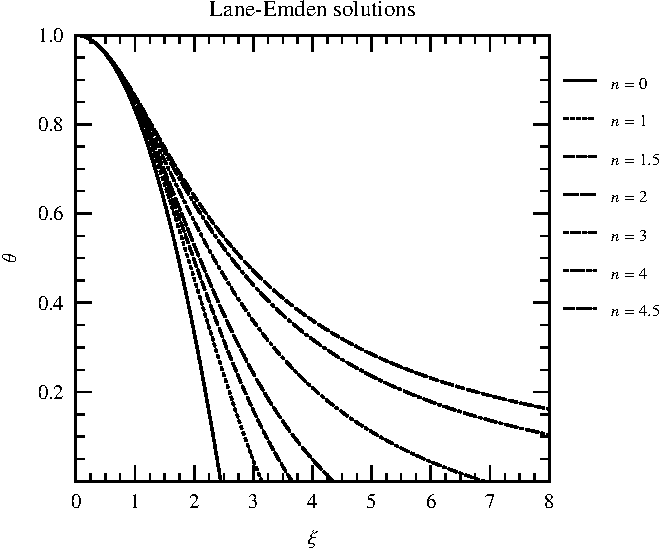
\includegraphics[width=4in]{LE_all.pdf}}
\caption{Solutions of the Lane-Emden equation for selected valued of the index $n$.}
\label{f.LE-solutions}
\end{figure}

\section{Some Useful Relations}

First, let's get the mass of our polytropic sphere.  To do this, we write the integral
\[ M = \int_{0}^{R} 4\pi r^{2} \rho\,\dif r \]
and make the substitutions $r = r_{n}\xi$, $R = r_{n}\xi_{1}$, and $\rho = \rho_{c}\theta^{n}(\xi)$ to obtain
\[
M = 4\pi r_{n}^{3}\rho_{c}\int_{0}^{\xi_{1}} \xi^{2}\theta^{n}(\xi)\,\dif\xi.
\]
Using equation~(\ref{e.LE}) , the integrand can be written as a perfect differential, so we get
\begin{equation}\label{e.LE-mass}
M = 4\pi r_{n}^{3} \rho_{c}\left(-\xi_{1}^{2} \theta_{1}'\right).
\end{equation}
Here I define the shorthand $\theta_{1}' \equiv \theta(\xi)|_{\xi=\xi_{1}}$.  Substituting $r_{n} = R/\xi_{1}$ and dividing by 3 allows us to get a formula relating the central density to the mean density,
\begin{equation}\label{e.LE-density-ratio}
\rho_{c} = \frac{3M}{4\pi R^{3}}\left(-\frac{\xi_{1}}{3\theta_{1}'}\right).
\end{equation}
For the solutions shown in Figure~\ref{f.LE-solutions}, we have the following values of $\rho_{c}/\bar{\rho}$, as shown in Table~\ref{t.LE-properties}.
As the index $n$ increases, the configuration becomes more and more concentrated toward the center.

\begin{table}[htpb]
\caption{Properties of the Lane-Emden solutions.\label{t.LE-properties}}
\begin{tabular}{c|rrrrrrr}
\hline
$n$ & 0 & 1.0 & 1.5 & 2.0 & 3.0 & 4.0 & 4.5 \\
\hline\hline
$\xi_{1}$ & 2.449 & 3.142 & 3.654 & 4.353 & 6.897 & 14.972 & 31.836\\
$-\theta_{1}'$ & 0.8165 & 0.3183 & 0.2033 & 0.1272 & 0.04243 & 0.008018 & 0.001715\\
$\rho_{c}/\bar{\rho}$ & 1.00 & 3.29 & 5.99 & 11.41 & 54.18 & 622.4 & 6187.8\\
\hline
\end{tabular}
\end{table}

Starting from equation~(\ref{e.LE-mass}), we can substitute for $r_{n}$ using equation~(\ref{e.LE-length-scale}) and $\rho_{c}$ using equation~(\ref{e.LE-density-ratio}) to get an equation for the central pressure,
\begin{equation}\label{e.LE-PC}
P_{c} = \frac{GM}{R^{4}} \frac{1}{4\pi(n+1)(-\theta_{1}')^{2}}.
\end{equation}
For an ideal gas, $P_{c} = (\NA\kB/\mu)\rho_{c}T_{c}$ with $\mu$ being the mean molecular weight, we can solve for the central temperature,
\begin{equation}\label{e.LE-TC}
T_{c} = \left(\frac{\mu}{\NA\kB}\right)\left(\frac{GM}{R}\right)\frac{1}{(n+1)\xi_{1}(-\theta_{1}')}.
\end{equation}
Finally, starting from equation~(\ref{e.LE-PC}), substituting for $P_{c}$ using equation~(\ref{e.polytope}), and eliminating $\rho_{c}$ using equation~(\ref{e.LE-density-ratio}), we obtain a relation between mass and radius in terms of $K$ and $n$,
\begin{equation}\label{e.LE-mass-radius}
M^{1-1/n} = \left[\frac{K(n+1)}{G(4\pi)^{1/n}} \xi_{1}^{1+1/n}\left(-\theta_{1}'\right)^{1-1/n} \right] R^{1-3/n}.
\end{equation}
Alternatively, one could use this equation to fit $K$ to a star of known $M$ and $R$.

Finally, we can derive a formula for the gravitational energy of our polytropic sphere.  First, we can integrate the equation for the energy,
\[
E_{\mathrm{grav}} = -G\int_{0}^{M}\frac{m}{r}\,\dif m,
\]
by parts to obtain
\begin{equation}\label{e.polytrope-energy-1}
E_{\mathrm{grav}} = -\frac{GM^{2}}{2R} - \frac{1}{2}\int_{0}^{R}\frac{Gm^{2}}{r^{2}}\,\dif r = -\frac{GM^{2}}{2R} - \frac{1}{2}\int_{0}^{R} \frac{\dif\Phi}{\dif r} m\,\dif r.
\end{equation}
If we define our zero of energy to be such that $\Phi(R) = 0$, then we can integrate by parts again to obtain
\begin{equation}\label{e.polytrope-energy-2}
E_{\mathrm{grav}} = -\frac{GM^{2}}{2R} + \frac{1}{2}\int_{0}^{R} \Phi\,\dif m.
\end{equation}
We can rewrite the equation of hydrostatic equilibrium as
\[ \frac{\dif P}{\dif r} = -\frac{\dif\Phi}{\dif r} \rho \]
and use equation~(\ref{e.polytope}) to eliminate $P$ to obtain
\[ \frac{\dif\Phi}{\dif r} = (1+n) K \rho^{1/n} .\]
Integrating from a point in the star $r$ to $R$, and again using choosing $\Phi(R) = 0$, we obtain
\begin{equation}\label{e.polytrope-energy-3}
\Phi(r) = -(1+n)K\rho(r)^{1/n} = -(1+n)K\frac{P(r)}{\rho(r)}.
\end{equation}
Inserting equation~(\ref{e.polytrope-energy-3}) into equation~(\ref{e.polytrope-energy-2}), we have
\begin{equation}\label{e.polytrope-energy-4}
E_{\mathrm{grav}} = -\frac{GM}{2R} - \frac{1+n}{2}\int_{0}^{M} \frac{P}{m}\,\dif m = -\frac{GM}{2R} - \frac{1+n}{6}E_{\mathrm{grav}},
\end{equation}
where we used equation~(\ref{e.virial-1}) to relate the integral of $P/\rho$ to $E_{\mathrm{grav}}$. Solving equation~(\ref{e.polytrope-energy-4}) for $E_{\mathrm{grav}}$ gives us the desired result,
\begin{equation}\label{e.polytrope-energy}
E_{\mathrm{grav}} = -\frac{3}{5-n} \frac{GM^{2}}{R}.
\end{equation}
Note that solutions with $n > 5$ have a positive gravitational energy.

\section{Exercises}\label{s.LE-exercises}
\begin{enumerate}
\item What is the index $n$ for a constant density star? For an isothermal star? For a star with a degenerate, non-relativistic equation of state? For a star in which radiation pressure dominates?

\item Derive equations~(\ref{e.LE-mass})--(\ref{e.LE-mass-radius}).

\item Explain what the mass-radius relation, eq.~(\ref{e.LE-mass-radius}), means for the cases $n=1$ and $n=3$.

\item For a fully convective star, how is the polytropic constant $K$ related to the entropy? Derive a formula for $R$ in terms of $M$ and $s$ in this case.  What happens to the star if heat is added to it?

\item Consider a polytrope of index $3/2$.
\begin{enumerate}
\item Using the expression for the entropy of an ideal gas (eq.~\ref{e.sacker-tetrode}]), show that the entropy is constant throughout the star in this case.
\item Use the Lane-Emden solution to compute the specific entropy, per unit mass, in terms of the central temperature $T$ and the stellar mass $M$: $s = s(T_{c},M)$.
\item Now compute the ``gravothermal'' specific heat
\begin{equation}\label{e.cstar}
c_{\star} = T_{c}\frac{\partial s(T_{c},M)}{\partial T_{c}},
\end{equation}
and comment on its physical significance.
\end{enumerate}

\item We will see later that low-mass pre-main-sequence stars are fully convective and have nearly constant effective temperatures.  Let's use these facts to estimate the timescale for contraction.  Assume $T_{\mathrm{eff}} = \mathrm{const.}$ and write the equation for energy balance as $L = -\dif E/\dif t$, where $E$ refers to the total energy of the pre-main-sequence star (Why is there a minus sign?).  
\begin{enumerate}
\item Starting from this equation, derive an equation for $R(t)$. What is the characteristic timescale for a star to contract? Scale your answer to $T_{\mathrm{eff}} = 3000\nsp\K$ and $M = 0.1\nsp\Msun$.  
\item Derive expressions for the central density $\rho_{c}(t)$ and temperature $T_{c}(t)$.
\item Using these results, calculate the time required to contract to a radius such that $\eF(\rho_{c}) = \kB T_{c}$, where $\eF$ is the Fermi energy?
\end{enumerate}
\end{enumerate}
